\documentclass{beamer}
\usepackage[latin9]{inputenc}
\usepackage{unicode}
\usepackage{hyperref}
\usepackage[austrian]{babel}
\usepackage[T1]{fontenc}
\usepackage[round]{natbib}
\usepackage{graphicx}
%\usepackage{subfigure}
\usepackage{C:/Programme/R/share/texmf/Sweave}
\usepackage{beamerthemesplit} % kam neu dazu


\begin{document}
\title{\textbf{Sch�tzung und Kalibrierung von Copulae}\\
  \emph{Welche Copula passt zu meinen Daten?} \\
  \footnotesize{Implementierung von Sch�tzungsmethoden f\"ur den bivariaten Fall in
  \emph{R}}
  }

\author{
  Gerold K�b (0250001)\\
  Martin Gartner (0351427)
}
\date{\today} 

\frame{\titlepage} 

\frame{\frametitle{Inhaltsverzeichnis}\tableofcontents} 

\section{Warum Copulae verwenden?}
%\subsection{Motivation} 
\frame{\frametitle{Motivation} 

Finanzm�rkte der Realit�t entsprechen h�ufig nicht den Annahmen der Finanzmarkttheorie, zB

	\begin{itemize}
	\item \textit{fat tails} der Verteilungen
	\item Korrelation von null bedeutet in Praxis nicht zwingend Unabh�ngigkeit
	\item Auftreten von Clustern in Volatilit�t
	\end{itemize}

Dies f\"uhrt zu Schwierigkeiten im Sch�tzen der gemeinsamen Verteilungsfunktion eines Portfolios.
}
%\subsection{Probleme gemeinsamer Verteilungsfunktionen}
\frame{\frametitle{Probleme gemeinsamer Verteilungsfunktionen}
Probleme:
\begin{itemize}
	\item Kann man VaR zweier Instrumente einfach addieren um VaR des Portfolios zu erhalten?
	\item Wie kann man Abh�ngigkeit innerhalb der Instrumente des Portfolios beschreiben?
	\item Pearson's Korrelation hat einige Nachteile
\end{itemize}

L�sung:
\begin{itemize}
	\item Mit Copulae kann Abh�ngigkeitsstruktur und gemeinsame Verteilung besser gesch�tzt werden!
\end{itemize}

}
\section{Copulae}
\subsection{Was ist eine Copula?}
\frame{\frametitle{Was ist eine Copula?}
Eine \emph{Copula} ist eine Funktion, die eine
multivariate Verteilungsfunktion mit ihren eindimensionalen
Randverteilungen kombiniert.

\begin{itemize}
	\item $X$, $Y$ \ldots zwei stetige Zufallsvariablen mit $F(x)~=~P(X \leq x)$ und $G(y) = P(Y \leq y)$
	\item gemeinsame Verteilung $H(x, y) = P(X \leq x, Y \leq y)$
	\item f\"ur $(x, y)~\in~[-\infty, \infty]^2$ gibt es Punkt $\left(F(x), G(y), H(x,y)\right)$
	\item \emph{Copula} ist nun die Abbildung von $\mathbf{I}^2$ nach $\mathbf{I}$
\end{itemize}
}

\frame{\frametitle{Interpretation als Volumen}
Darstellbar als Volumen in $\mathbf{I}^3$:
  \begin{figure}[htb]  
  	\centering
        %\label{fig:copulabounds}
        %\caption{Frechet-Hoeffding-Bounds}
    \begin{minipage}[b]{.3\textwidth} % [b] => Ausrichtung an \caption
      \caption{$W(x, y)$}
      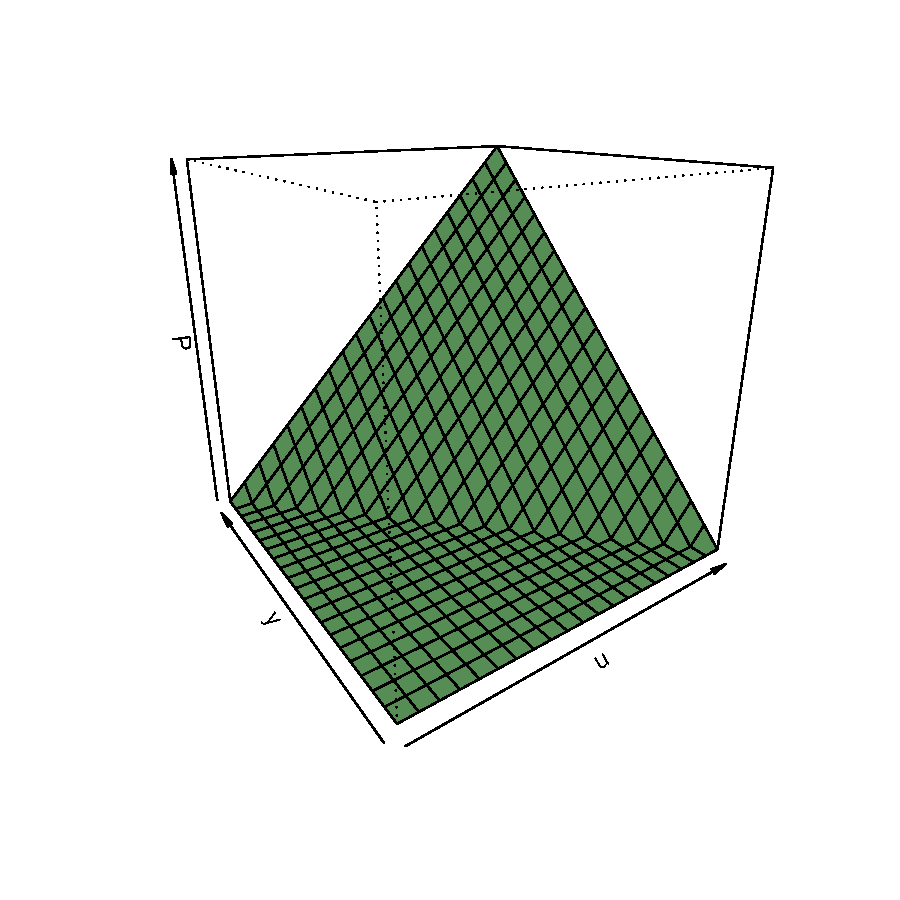
\includegraphics[width = \textwidth]{copulaM}
    \end{minipage}
    \hspace{.0\linewidth}% Abstand zwischen Bilder
    \begin{minipage}[b]{.3\textwidth} % [b] => Ausrichtung an \caption
      \caption{$\Pi(x, y)$}
      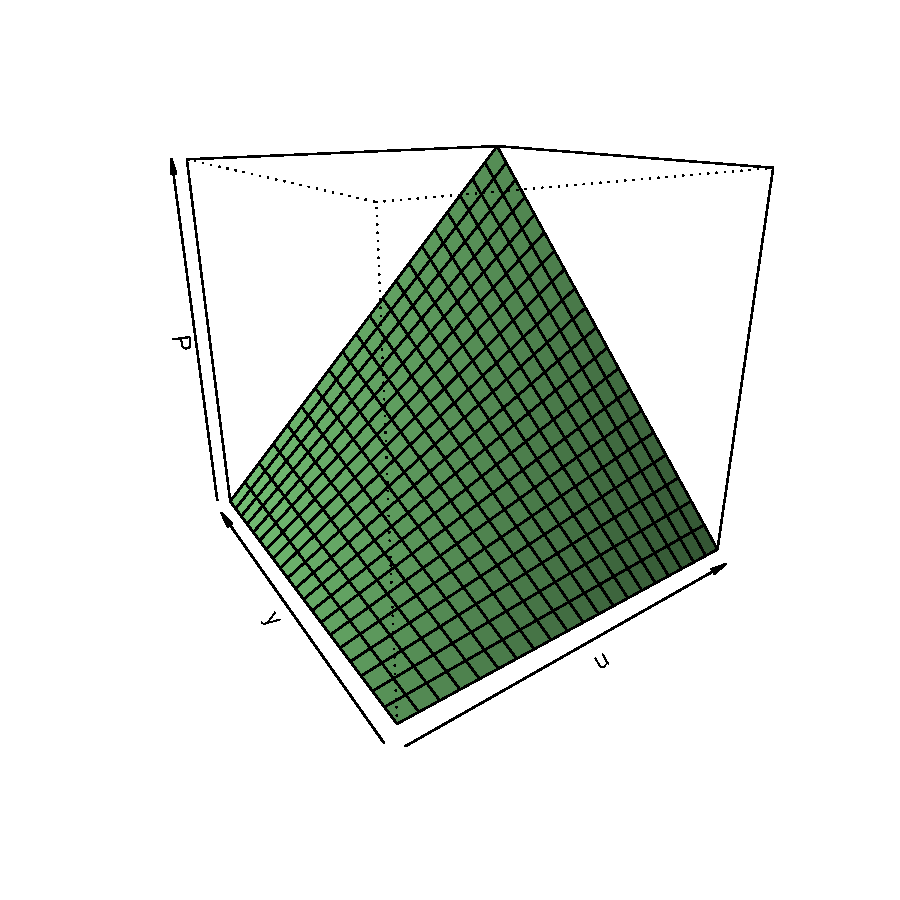
\includegraphics[width = \textwidth]{copulaPi}
    \end{minipage}
    \hspace{.0\linewidth}% Abstand zwischen Bilder
    \begin{minipage}[b]{.3\textwidth} % [b] => Ausrichtung an \caption
      \caption{$M(x, y)$}
      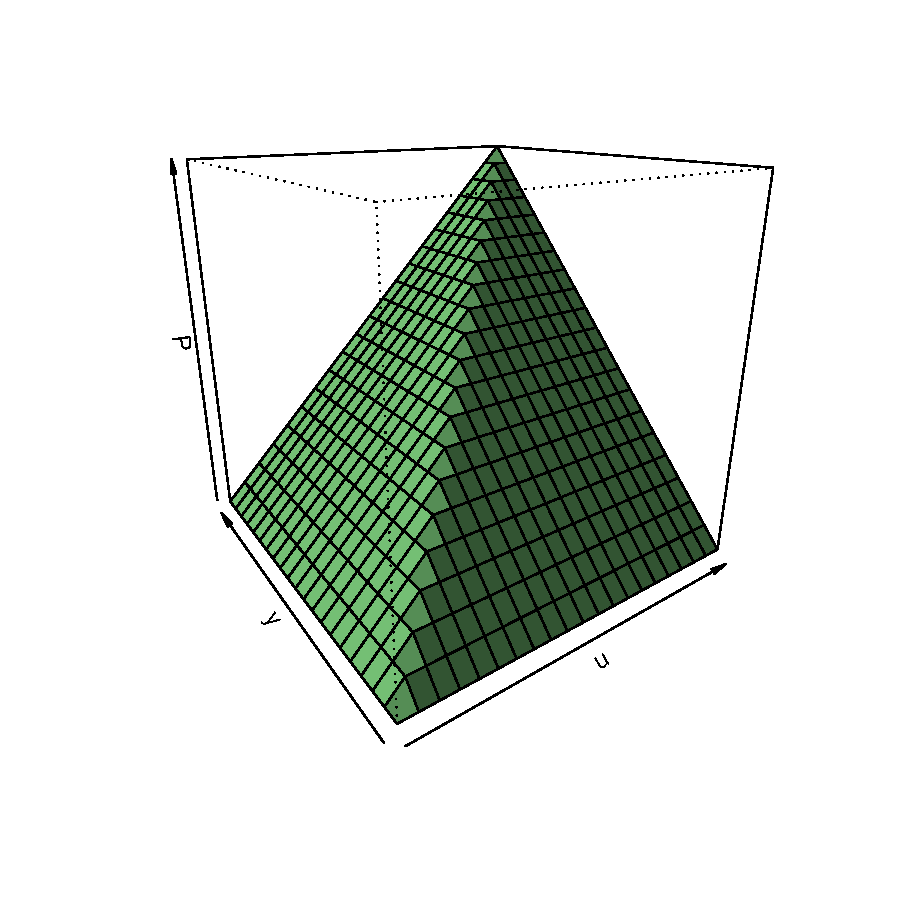
\includegraphics[width = \textwidth]{copulaW}
    \end{minipage}
  \end{figure}

und daher als Wahrscheinlichkeitskennzahl in $\mathbf{I}^2$ interpretierbar.
}

\subsection{Sklar's Theorem}
\frame{\frametitle{Sklar's Theorem}
Gemeinsame Verteilung kann durch die \emph{Copula} ausgedr\"uckt werden:
\begin{equation}
  \label{eq:sklar}
  H(x, y) = C(F(x), G(y))
\end{equation}
Gilt auch f\"ur den multivariaten Fall!\\~\\

Alle Copulae liegen zwischen zwei Grenzen. Seien $M$ und $W$ die Copulae
\begin{eqnarray}
  \label{eq:bounds}
  M(x, y) & = & \min{(x, y)} \\
  W(x, y) & = & \max{ (x + y - 1, 0)}
\end{eqnarray}
}

\subsection{Die Frech\'et-Hoeffding Bounds}
\frame{\frametitle{Eigenschaften von Copulae}
Es gilt
\begin{equation}
  \label{eq:frechethoeffding}
  W(x, y) \leq C(x, y) \leq M(x, y)
\end{equation}
  \begin{figure}[htb]  
  	\centering
        %\label{fig:copulabounds}
        %\caption{Frechet-Hoeffding-Bounds}
    \begin{minipage}[b]{.3\textwidth} % [b] => Ausrichtung an \caption
      \caption{$W(x, y)$}
      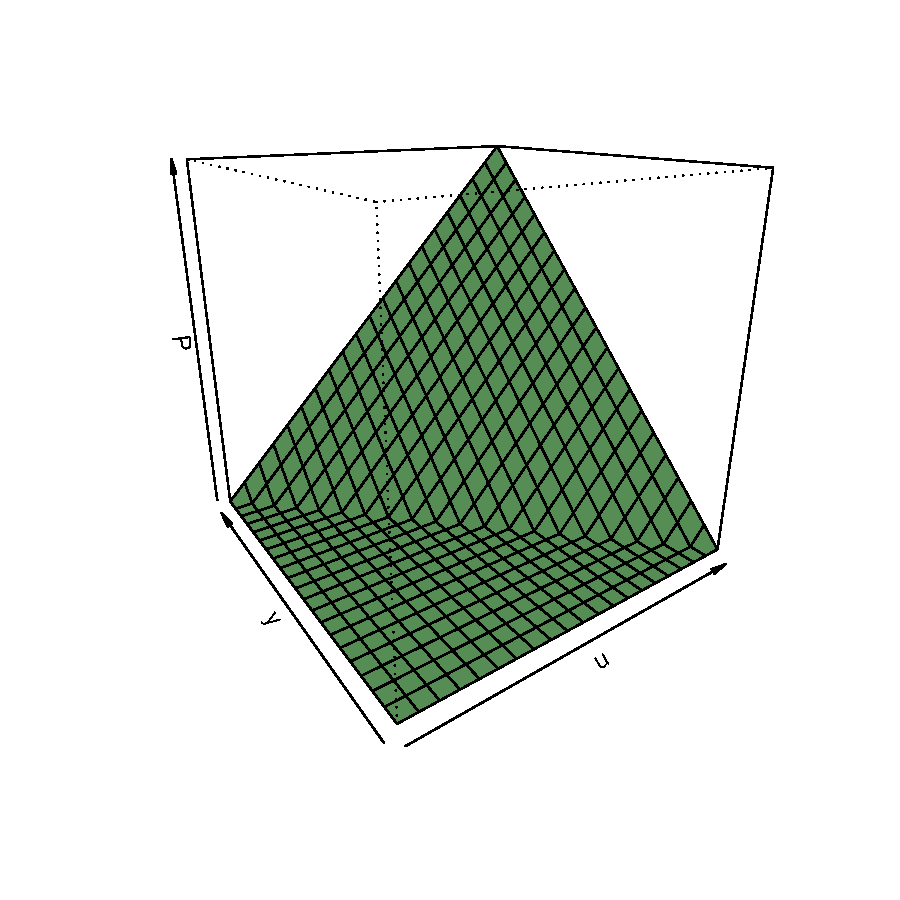
\includegraphics[width = \textwidth]{copulaM}
    \end{minipage}
    \hspace{.0\linewidth}% Abstand zwischen Bilder
    \begin{minipage}[b]{.3\textwidth} % [b] => Ausrichtung an \caption
      \caption{$\Pi(x, y)$}
      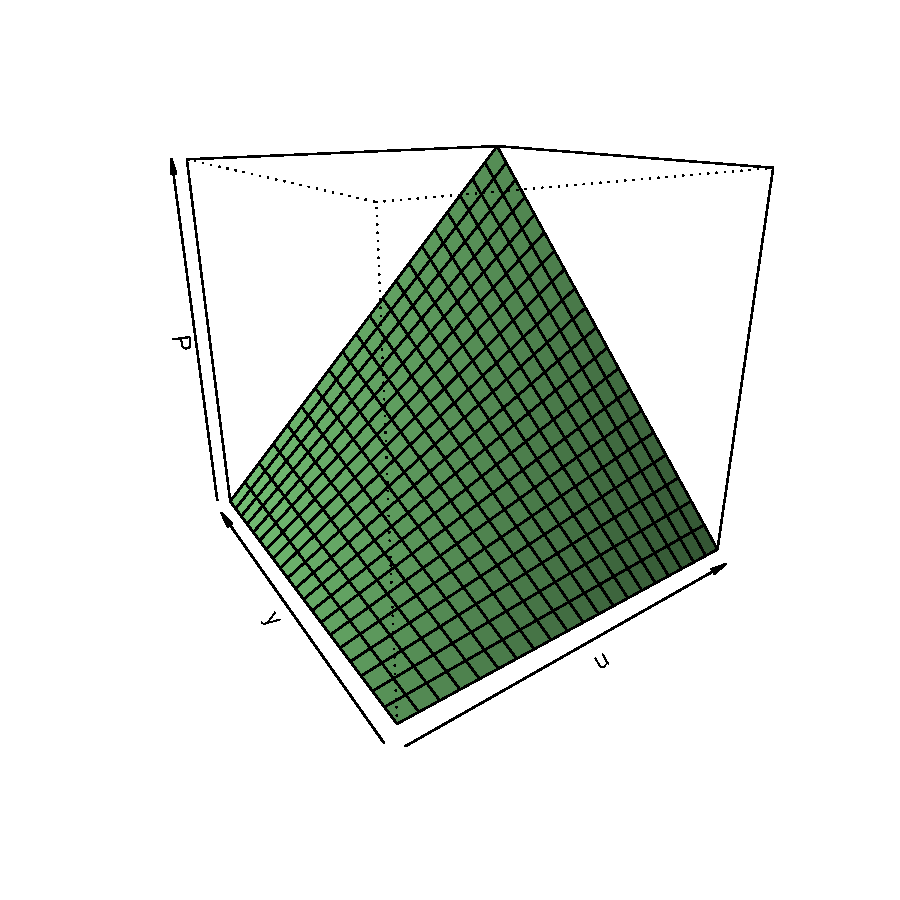
\includegraphics[width = \textwidth]{copulaPi}
    \end{minipage}
    \hspace{.0\linewidth}% Abstand zwischen Bilder
    \begin{minipage}[b]{.3\textwidth} % [b] => Ausrichtung an \caption
      \caption{$M(x, y)$}
      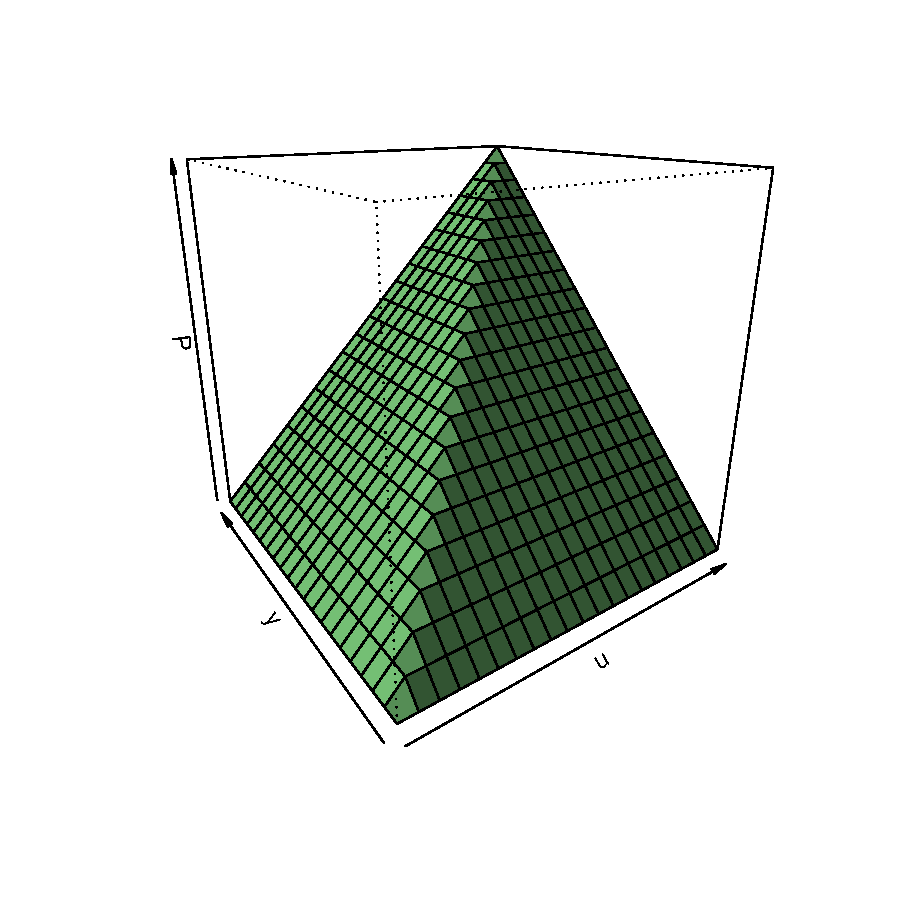
\includegraphics[width = \textwidth]{copulaW}
    \end{minipage}
  \end{figure}
}


\section{Familien von Copulae}
\frame{\frametitle{Familien von Copulae}

\begin{itemize}
\item 
  \begin{block}{Elliptische Copulae}
    \begin{itemize}
    \item Copulae von	elliptischen Verteilungen\
    \item zB beide Randverteilungen sind normal- oder t-verteilt
    \end{itemize}
  \end{block}
\item
  \begin{block}{Archimedische Copulae}
    \begin{itemize}
    \item einfach zu erzeugen
    \item viele parametrische Familien (22 nach Nelsen (2006))
    \item k�nnen an viele gew\"unschte Eigenschaften angepasst werden
    \end{itemize}
  \end{block}
\end{itemize}

}

\subsection{Elliptische Copulae}
\frame{\frametitle{Elliptische Copulae f\"ur n = 2}
\begin{itemize}
	\item Gau�'sche Copula
		\small{
				\begin{equation}
				  C_G(u,v) = \int_{-\infty}^{\Phi^{-1}(u)}
				  \int_{-\infty}^{\Phi^{-1}(v)} \frac{1}{2 \pi \sqrt{(1 - \rho^2)}}
				  \exp{ \left( -\frac{s^2 - 2 \rho s t + t^2} {2 (1 - \rho^2)}
				    \right) }ds dt
				\end{equation}
			}
	\item T-Copula
		\small{
						\begin{equation}
						  C_t(u, v) = \int_{-\infty}^{t_{\nu}^{-1}(u)}
						  \int_{-\infty}^{t_{\nu}^{-1}(v)} \frac{1}{2 \pi \sqrt{(1 - \rho^2)}}
						  \exp{ \left( -\frac{s^2 - 2 \rho s t + t^2} {2 (1 - \rho^2)}
						    \right) }ds dt
						\end{equation}
				}
\end{itemize}
}



\section{Bl�cke}
\subsection{Bl\"ocke}
\frame{\frametitle{Bl\"ocke}

\begin{block}{Blocktitel}
Blocktext 
\end{block}

\begin{exampleblock}{Blocktitel}
Blocktext 
\end{exampleblock}


\begin{alertblock}{Blocktitel}
Blocktext 
\end{alertblock}
}
\end{document}